\documentclass[border=4pt]{standalone}
\usepackage[T1]{fontenc}
\usepackage{lmodern}
\usepackage{amsmath}
\usepackage{pgfplots}
\pgfplotsset{compat=1.18}
\usepgfplotslibrary{groupplots,fillbetween}
\usetikzlibrary{calc,arrows.meta}
% one colour per kind of method, the same in every figure (Okabe-Ito)
\definecolor{neur}{HTML}{D55E00}   % neurons chosen by attribution
\definecolor{dirc}{HTML}{009E73}   % directions from the weird-vs-normal contrast
\definecolor{read}{HTML}{0072B2}   % readout methods and interventions chosen from readouts
\definecolor{pers}{HTML}{CC79A7}   % Assistant Axis / persona
\definecolor{ctrl}{HTML}{8C8C8C}   % random controls
\definecolor{meas}{HTML}{E69F00}   % measured outcome
\definecolor{ink}{HTML}{222222}
\pgfplotsset{
  every axis/.append style={clip=false, font=\small, axis line style={black!55}, tick style={black!55}, tick align=outside,
    label style={font=\small}, tick label style={font=\footnotesize}, title style={font=\small, align=center}},
  grid style={black!9, line width=0.4pt},
  every axis legend/.append style={font=\footnotesize, draw=none, fill=none},
  ci/.style={/pgfplots/error bars/x dir=both, /pgfplots/error bars/x explicit, /pgfplots/error bars/error bar style={line width=0.8pt}, /pgfplots/error bars/error mark=none},
  yci/.style={/pgfplots/error bars/y dir=both, /pgfplots/error bars/y explicit, /pgfplots/error bars/error bar style={line width=0.8pt}, /pgfplots/error bars/error mark=none},
}

\begin{document}
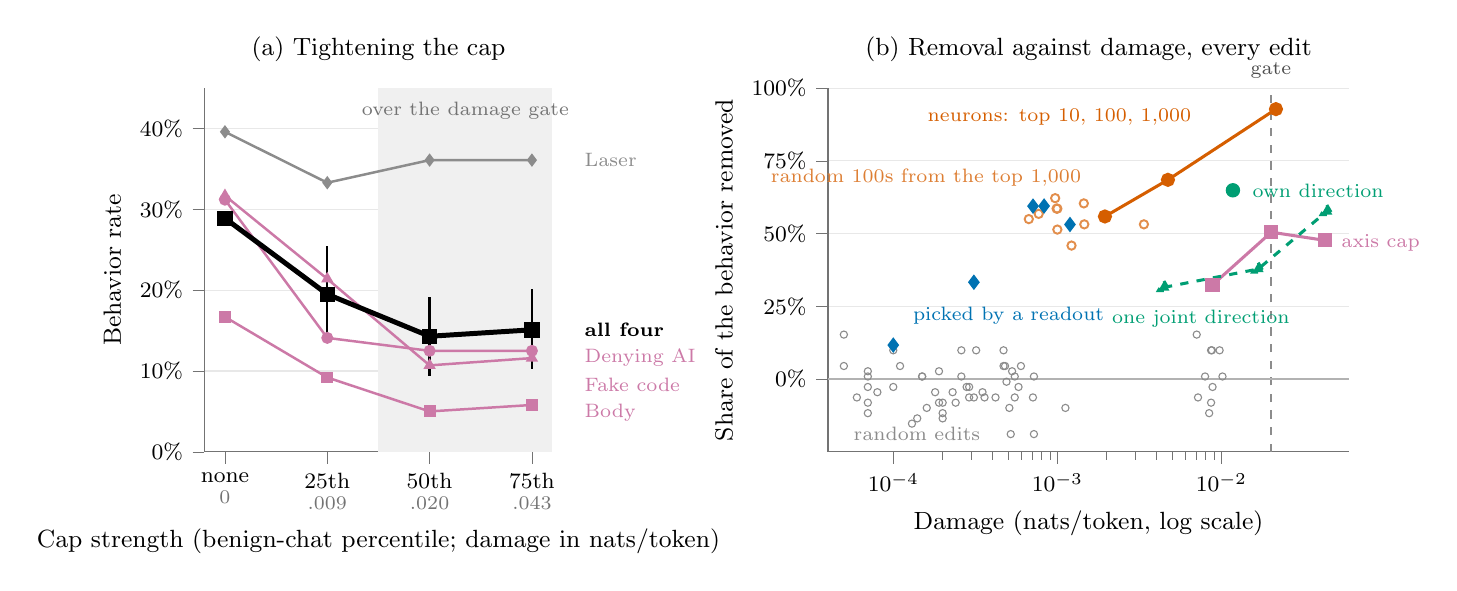
\begin{tikzpicture}
\begin{groupplot}[group style={group size=2 by 1, horizontal sep=3.5cm}, height=6.2cm, axis x line*=bottom, axis y line*=left, ymajorgrids]
\nextgroupplot[width=6.0cm, xmin=-0.2, xmax=3.2, xtick={0,1,2,3}, xticklabels={{none\\[-2pt]{\scriptsize\color{black!55}0}},{25th\\[-2pt]{\scriptsize\color{black!55}.009}},{50th\\[-2pt]{\scriptsize\color{black!55}.020}},{75th\\[-2pt]{\scriptsize\color{black!55}.043}}}, xticklabel style={align=center}, ymin=0, ymax=45, ytick={0,10,20,30,40}, yticklabel={$\pgfmathprintnumber{\tick}\%$}, ylabel={Behavior rate}, xlabel={Cap strength (benign-chat percentile; damage in nats/token)}, title={(a) Tightening the cap}]
\fill[black!6] (axis cs:1.5,0) rectangle (axis cs:3.2,45);
\node[font=\scriptsize, black!55, anchor=north] at (axis cs:2.35,44.5) {over the damage gate};
\addplot[pers, line width=0.9pt, mark=*, mark size=1.7pt] coordinates {(0,31.20) (1,14.10) (2,12.50) (3,12.50)};
\addplot[pers, line width=0.9pt, mark=square*, mark size=1.7pt] coordinates {(0,16.70) (1,9.20) (2,5.00) (3,5.80)};
\addplot[pers, line width=0.9pt, mark=triangle*, mark size=1.7pt] coordinates {(0,31.70) (1,21.40) (2,10.70) (3,11.60)};
\addplot[ctrl, line width=0.9pt, mark=diamond*, mark size=1.7pt] coordinates {(0,39.60) (1,33.30) (2,36.10) (3,36.10)};
\addplot[black, line width=1.8pt, mark=square*, mark size=1.9pt, yci] coordinates {(0,28.90) += (0,0.00) -= (0,0.00) (1,19.50) += (0,6.00) -= (0,5.40) (2,14.30) += (0,4.90) -= (0,4.90) (3,15.10) += (0,5.00) -= (0,4.90)};
\node[font=\scriptsize, ctrl, anchor=west] at (axis cs:3.42,36.10) {Laser};
\node[font=\scriptsize, black, anchor=west] at (axis cs:3.42,15.10) {\textbf{all four}};
\node[font=\scriptsize, pers, anchor=west] at (axis cs:3.42,11.70) {Denying AI};
\node[font=\scriptsize, pers, anchor=west] at (axis cs:3.42,8.30) {Fake code};
\node[font=\scriptsize, pers, anchor=west] at (axis cs:3.42,4.90) {Body};
\nextgroupplot[width=8.2cm, xmode=log, xmin=4e-5, xmax=0.06, xtick={1e-4,1e-3,1e-2}, xticklabels={$10^{-4}$,$10^{-3}$,$10^{-2}$}, ymin=-25, ymax=100, ytick={0,25,50,75,100}, yticklabel={$\pgfmathprintnumber{\tick}\%$}, xlabel={Damage (nats/token, log scale)}, ylabel={Share of the behavior removed}, title={(b) Removal against damage, every edit}]
\draw[black!45, dashed, line width=0.7pt] (axis cs:0.02,-25) -- (axis cs:0.02,100) node[above, font=\scriptsize, black!70] {gate};
\draw[black!30, line width=0.5pt] (axis cs:4e-5,0) -- (axis cs:0.06,0);
\addplot[only marks, mark=o, mark size=1.3pt, ctrl] coordinates {(0.000230,-4.50) (0.000470,9.90) (0.000070,2.70) (0.000720,0.90) (0.000260,0.90) (0.000070,0.90) (0.000160,-9.90) (0.000490,-0.90) (0.000310,-6.30) (0.000350,-4.50) (0.000550,-6.30) (0.000480,4.50) (0.000130,-15.30) (0.000600,4.50) (0.000150,0.90) (0.000520,-18.90) (0.000100,9.90) (0.000470,4.50) (0.000280,-2.70) (0.000720,-18.90) (0.000510,-9.90) (0.000070,-2.70) (0.000190,2.70) (0.000050,15.30) (0.000420,-6.30) (0.000050,4.50) (0.000070,-8.10) (0.000710,-6.30) (0.001120,-9.90) (0.000200,-8.10) (0.010150,0.90) (0.007070,15.30) (0.008650,9.90) (0.007200,-6.30) (0.007950,0.90) (0.008830,-2.70) (0.009750,9.90) (0.008420,-11.70) (0.008750,9.90) (0.008650,-8.10) (0.000200,-13.50) (0.000240,-8.10) (0.000140,-13.50) (0.000290,-2.70) (0.000180,-4.50) (0.000200,-11.70) (0.000530,2.70) (0.000150,0.90) (0.000320,9.90) (0.000290,-6.30) (0.000190,-8.10) (0.000100,-2.70) (0.000080,-4.50) (0.000070,-11.70) (0.000110,4.50) (0.000550,0.90) (0.000060,-6.30) (0.000360,-6.30) (0.000260,9.90) (0.000580,-2.70)};
\addplot[only marks, mark=o, mark size=1.5pt, neur!70, line width=0.7pt] coordinates {(0.001220,45.90) (0.001460,53.20) (0.003370,53.20) (0.001000,58.60) (0.000970,62.20) (0.000670,55.00) (0.001000,51.40) (0.000770,56.80) (0.001450,60.40) (0.000990,58.60)};
\addplot[neur, line width=1.1pt, mark=*, mark size=2pt] coordinates {(0.001950,55.90) (0.004720,68.50) (0.021490,92.80)};
\addplot[pers, line width=1.1pt, mark=square*, mark size=2pt] coordinates {(0.008830,32.40) (0.020140,50.50) (0.042590,47.70)};
\addplot[dirc, line width=1.1pt, mark=triangle*, mark size=2.3pt, dashed] coordinates {(0.004464,31.53) (0.016758,37.84) (0.043895,57.66)};
\addplot[only marks, dirc, mark=*, mark size=2.4pt] coordinates {(0.011750,64.90)};
\addplot[only marks, read, mark=diamond*, mark size=2.5pt] coordinates {(0.000100,11.70) (0.000310,33.30) (0.000830,59.50) (0.001194,53.15) (0.000711,59.46)};
\node[font=\scriptsize, neur, anchor=east] at (axis cs:0.0075,90) {neurons: top 10, 100, 1,000};
\node[font=\scriptsize, neur!80, anchor=south east] at (axis cs:0.0016,63) {random 100s from the top 1,000};
\node[font=\scriptsize, read, anchor=north west] at (axis cs:1.15e-4,28) {picked by a readout};
\node[font=\scriptsize, pers, anchor=west] at (axis cs:0.047,47) {axis cap};
\node[font=\scriptsize, dirc, anchor=west] at (axis cs:0.013512,64.90) {own direction};
\node[font=\scriptsize, dirc, anchor=north] at (axis cs:0.0075,27) {one joint direction};
\node[font=\scriptsize, ctrl, anchor=north west] at (axis cs:5e-5,-13) {random edits};
\end{groupplot}
\end{tikzpicture}
\end{document}
